\section{Methodology}\label{sec:method-ML}
This section presents the experiments done with machine learning techniques to predict GPU kernels. Two different approaches with machine learning were proposed. First approach was done with the same features than analytical model, trying to be fair with the analytical model; and second approach was done using a phase of features extraction. 

The methodology of the first approach is shown in Section~\ref{ssec:methodFair} and the methodology of the second approach is presented in Section~\ref{ssec:methodExrtact}. 
In the second approach was used correlation analysis and hierarchical clustering to select the features to use a input in the machine learning algorithms. Profile information was collected of each Application over each GPU. 
We used three different machine learning methods: Linear Regression, Support Vector Machines and Random Forest. 
There exists other machine learning techniques with sophisticated learning process. However, in this work, we wanted to use simple models to prove that they achieve reasonable predictions.

The error of the predictions is presented using the Mean Absolute Percentage Error (MAPE), see equation~\ref{ec:MAPE}. In this equation, $t_m$ is the measured time and $t_k$ is the predicted time. With this error we have analysed the reliability of our approaches. 

\begin{equation}
    mape = \frac{100}{n}\sum _{t=1}^{n}\left|{\frac {{t_m}-{t_k}}{{t_m}}}\right| \label{ec:MAPE}
\end{equation}

We used R to automate the statistical analyses, in conjunction with the \texttt{e1071} and \texttt{randomForest} packages to use the \texttt{svm} and \texttt{randomForest} functions respectively. Collected data, experimental results and source codes are publicly available\footnote{Hosted at GitHub: \texttt{\scriptsize https://github.com/marcosamaris/gpuperfpredict} [Accessed on 6 march 2018]} under Creative Commons Public License. 

To perform our experiments with machine learning techniques, we first collected the performance profiles (metrics and events) for each kernel and GPU. 
All data was collected using the CUDA profiling tool \textbf{nvprof}. This profiling tool enables us to collect data from the command-line reducing the overhead of this process. This process is done without modifications on application source codes. nvprof has four modes to collect information from command-line: summary mode, GPU-trace/API-trace mode, event/metric summary mode and event/metric trace mode. We have used GPU-trace mode and event/metric trace mode.

GPU-trace mode permits collecting data only from CUDA API functions, such as kernel executions, memory transfer throughput between CPU and GPU, among others, without the overhead of profiling the main instructions. Execution times were collected in this mode, along with other features, such as CUDA grid and block dimensions, number of registers per thread, static and dynamic shared memory, device information, streams and the name of executed kernels. A total of 16 features were collected in this mode. 

In event/metric trace mode, all events and metrics are collected for each kernel execution. Although this causes a large overhead in the execution of the kernels, it gives detailed information about the behavior and performance of the executed CUDA kernel functions. All applications were iterated over their selected parameters. The number of events and metrics varied according to the compute capability of the GPUs. All collected information resulted in an approximated size of 12.5GB and the process spent up to 14 days in each GPU. 

For each sample, the metrics, events and traces information were collected in different phases, therefore avoiding the overhead over the measured execution time of the application. The execution time was taken from GPU-trace mode, thus each GPU-trace was executed ten times, and for the experiments was taken the mean of these samples and it was with a confidence interval of 95\%. 


\subsection{Machine Learning without extraction features}\label{ssec:methodFair}
These experiments were done with all the kernels presented in Section~\ref{ssec:useCases}, we used the two-dimensional applications (matrix multiplication and matrix addition) using three different sizes for the CUDA thread blocks, $8^2$, $16^2$ and $32^2$, and input sizes or matrix sizes we vary from $2^{8}$ to $2^{13}$ increasing the matrix size in a step of $2^8$. We took 32 samples per block size, resulting in 96 samples per GPU and a total of 768 samples. For the uni-dimensional problems (dot product and vector addition), the number of thread blocks also was varied in three configurations, $8^2$, $16^2$ and $32^2$, and we used input sizes or vector sizes from $2^{17}$ to $2^{28}$. From $2^{17}$ to $2^{22}$ 6 samples were taken, and from $2^{23}$ to $2^{28}$ 63 samples were taken. For these two applications 69 samples for each configuration were taken, resulting in 207 samples per GPU and a total of 1656 samples. For sub-array maximum problem, 69 samples with the original configuration were taken, for a total of 552 samples. 

All Rodinia applications were iterated over their selected parameters shown in Table~\ref{tab:GPUs}. For most kernels of Rodinia applications, we generated many samples, but we could generate only 57 samples on each GPU from the Back-Propagation (BCK) application. To limit the bias on the learning algorithms, we selected 100 random samples from the other applications in both approaches. It was, this sampled data, that was used as dataset for the ML algorithms in both approaches. 

To be fair with the analytical model, we then choose similar communication and computation parameters to use as feature inputs for the machine learning algorithms. We performed the evaluation using cross-validation, that is, for each target GPU, we performed the training using the other 8 GPUs, testing the model in the target GPU. This process was done for each application separately.

To compare fairly our analytical model with each ML techniques, the features that we used to feed the Linear Regression, Support Vector Machines and Random Forest algorithms are presented in Table \ref{tab:predictors}.

\begin{table}[htpb]
    \centering
    \scalebox{.825}{
        \begin{tabular}{c  c} 
        \toprule
        \textbf{Feature}&\textbf{Description} \\\midrule
        \texttt{num\_of\_cores} & \specialcell{Number of cores per GPU} \\ \midrule
        \texttt{max\_clock\_rate} & \specialcell{GPU Max Clock rate} \\\midrule
        \texttt{Bandwidth} & \specialcell{Theoretical Bandwidth} \\\midrule
        \texttt{Input Size} & \specialcell{Size of the problem} \\\midrule
        \texttt{totalLoadGM} & \specialcell{Load transaction in Global Memory} \\\midrule
        \texttt{totalStoreGM} & \specialcell{Store transaction in Global Memory} \\\midrule
        \texttt{TotalLoadSM} & \specialcell{Load transaction in Shared Memory} \\\midrule
        \texttt{TotalStoreSM} & \specialcell{Store transaction in Global Memory} \\\midrule
        \texttt{FLOPS SP} & \specialcell{Floating operation in Single Precision} \\\midrule
        \texttt{BlockSize} & \specialcell{Number of threads per blocks} \\\midrule
        \texttt{GridSize} & \specialcell{Number of blocks in the kernel} \\\midrule
        \texttt{No. threads} & \specialcell{Number of threads in the applications } \\\midrule
        % \texttt{Executed IPC} & \specialcell{Instructions executed per cycle} \\\midrule
        \texttt{Achieved Occupancy } & \specialcell{Ratio of the average active warps per active cycle to the maximum number of warps ed on a multiprocessor.} \\\midrule
        \end{tabular}}
        \caption{Features used as input in the machine learning techniques}
    \label{tab:predictors} 
\end{table}

To generate the flags \texttt{totalLoadGM}, \texttt{totalStoreGM}, \texttt{TotalLoadSM} and \texttt{TotalStoreSM}, the number of requests was divided by the number of transactions per request.

We first transformed the data to a $log_2$ scale and, after performing the learning and predictions, we returned to the original scale using a $2^{pred}$ transformation~\citep{Barnes:2008:RAS}, reducing the non-linearity effects. Figure~\ref{fig:QQplot} shows the difference between the trained model without (left-hand side graph) and with (right-hand side graph) logarithmic scale. The linear regression resulted in poor fitting in the tails, resulting in poor predictions. This problem was solved with the $log_2$ transformation.

\begin{figure}[htpb]
 \centering
 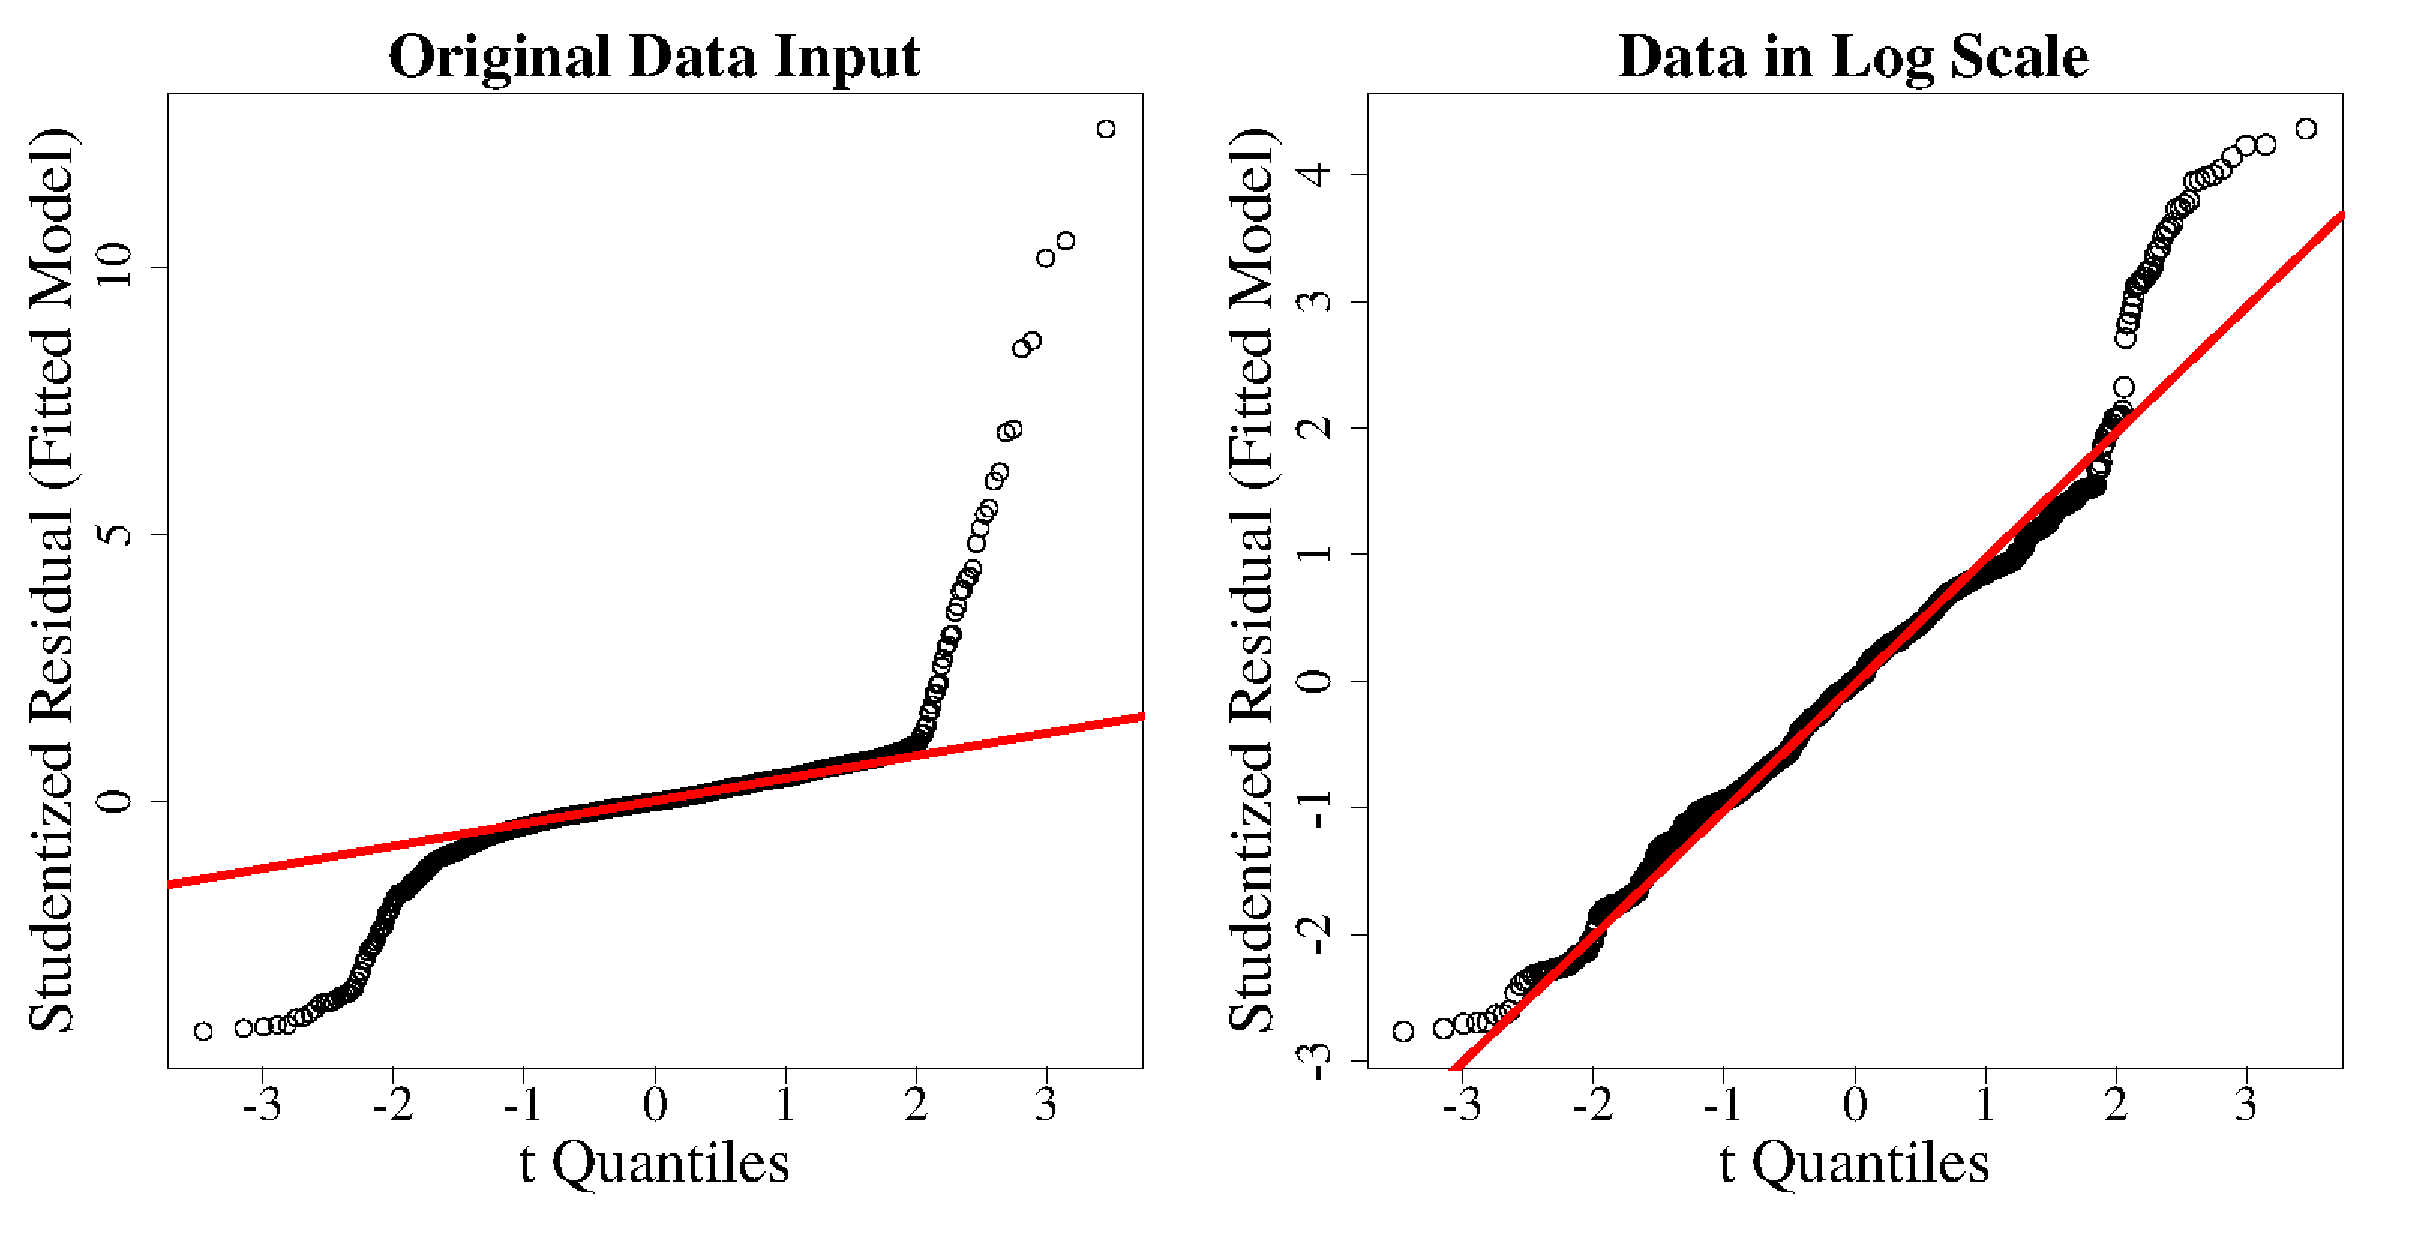
\includegraphics[scale=.3]{./images/QQplot.eps}
 \caption{Quantile-Quantile Analysis of the generated models}
 \label{fig:QQplot}
\end{figure}


\subsection{ML with extraction features}\label{ssec:methodExrtact}

In a machine learning process, the accuracy of the predictions depends on the quality of the pre-processing phase~\citep{Dasu:2003:EDM:861869}. In this section, we present a extraction features process to determine a set of parameters that permits predicting the running time of GPU applications in different contexts or scenarios. As it was mentioned above, we collected separately the set of events and metrics and the execution times of each application of Section~\ref{ssec:useCases} over all GPUs presented in Section~\ref{ssec:GPUTestbed}. 

To do these experiments, kernels of matrix addition, dot product, vector addition and sub-array maximum problem were used. The same number of samples than last section was used. All Rodinia applications were used. As before was mentioned, to limit the bias on the learning algorithms, we selected 100 random samples from the other applications. In total 16 kernels were used for these experiments. It was, this sampled data, that was used as dataset for the ML algorithms. 

We cleaned the collected information, dropping features with no variation among executions and without concordance among GPUs. Each cleaned sample of the dataset resulted in 85 kernel features plus 11 GPU architecture features, for a total of 96 features. We then performed a correlation analysis, followed by a clustering analysis to reduce the number of features (dimensionality reduction). 

We first transformed the data into a $log_2$ scale and, followed by a normalization, reducing the non-linearity effects~\citep{Barnes:2008:RAS} (line 2 and 3 of Algorithm~\ref{fig:methods}). To select a small number of application execution features to use with the ML algorithms, we performed correlation and clustering analyses over the data. We performed the correlation analysis using the Spearman Correlation Coefficient (SCC), since it captures relations and variations among features over different scales by using the rank values of the features. We evaluated the SCC for all features against the kernel execution times and applied a threshold of 0.75, keeping only the 21 features that had a SCC above it (line 4). These features are shown below:

\begin{algorithm}[htpb]
\SetAlgoLined
\KwResult{Prediction of the ML techniques}
\textbf{Input: Data sets}\;
ScaledData = scaleLog(Data sets)\;
NormalizedData = Normalize(ScaledData)\;
SCC = corr(NormalizedData, 0.75)\;
    \ForAll{No. Param in [5, 10]}{
    dendroG = hclust(corr(SCC))\;
    cutDendro = cutTree(dendroG, No. Param)\;
    features = variance(cutDendro)\;
        \ForAll{context in [GPUs, Kernels]}{
        \ForAll{ML in [LM, SVM, RF]}{
        trainingSet != features[context]\;
        testSet == features[context]\;
        
        Model = ML( trainingSet)\;
        output = predict(testSet)\;
        }
     }
 }
\caption{Algorithm of the methodological process done in this second approach} 
\label{fig:methods}
\end{algorithm}

\begin{lstlisting}[basicstyle=\small, numbers=none]
 [1] "elapsed_cycles_sm"                 
 [2] "gld_inst_32bit"                    
 [3] "gst_inst_32bit"                    
 [4] "inst_executed"                     
 [5] "inst_issued1"                      
 [6] "gld_request"                       
 [7] "gst_request"                       
 [8] "active_cycles"                     
 [9] "global_load_transactions"          
[10] "global_store_transactions"         
[11] "device_memory_read_transactions"   
[12] "l2_read_transactions"              
[13] "l2_write_transactions"             
[14] "issued_control.flow_instructions"  
[15] "executed_control.flow_instructions"
[16] "issued_load.store_instructions"    
[17] "executed_load.store_instructions"  
[18] "issue_slots"                       
[19] "control.flow_instructions"         
[20] "load.store_instructions"           
[21] "misc_instructions"  
\end{lstlisting}

To further reduce the features, we used a hierarchical clustering algorithm. We first create a similarity matrix over all features, using the Spearman correlation coefficient. This similarity matrix is the input for the clustering algorithm. This algorithm them performs the hierarchical clustering by first assigning each feature to its own cluster, and then proceeding iteratively, at each stage joining the two most similar clusters, continuing until there is just a single cluster, as shown in Figures~\ref{fig:Cuthclust:5} and \ref{fig:Cuthclust:10}, which present dendrograms built from 20 features. 

\begin{figure}[htbp]
    \centering
    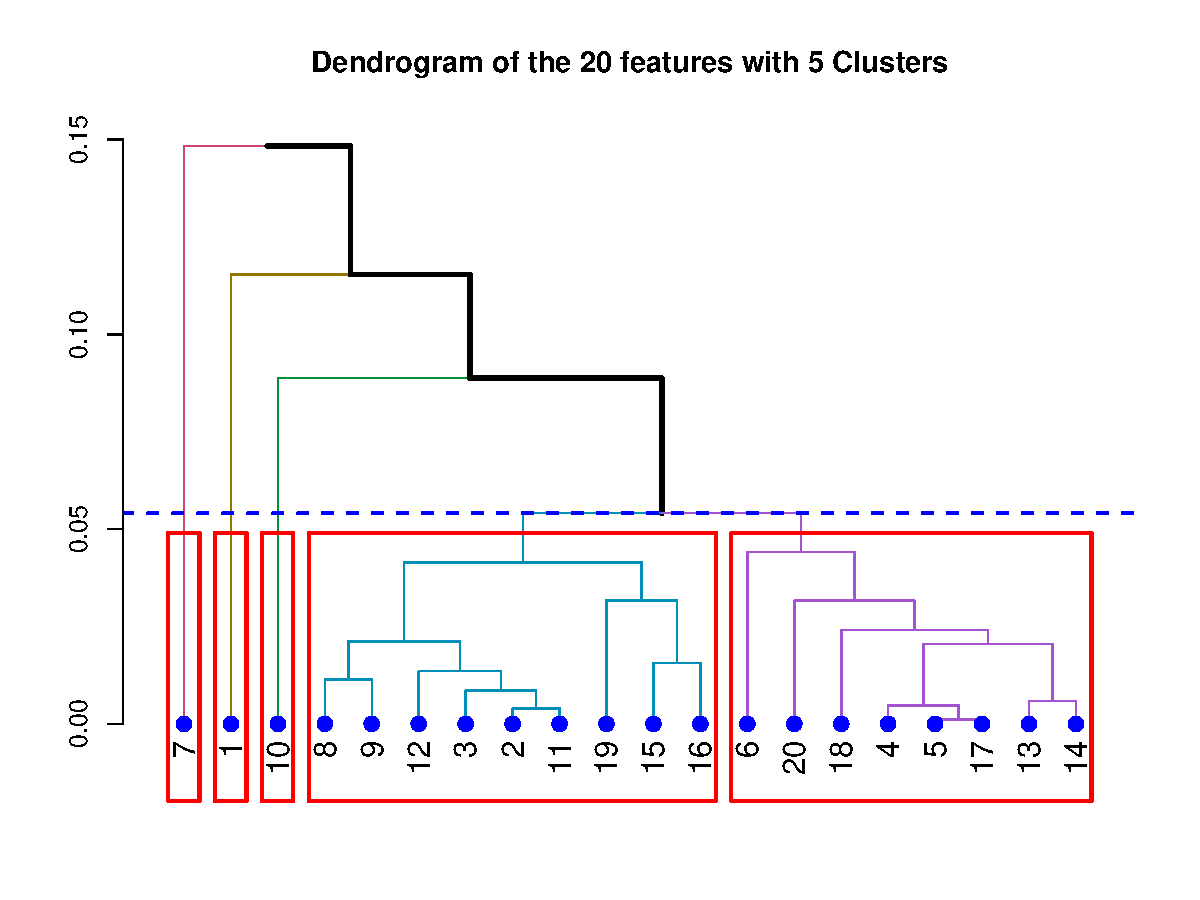
\includegraphics[scale=.75]{./images/cluster-5.pdf}
    \caption{Dendrogram with 5 clusters to select 1 features from each one}
    \label{fig:Cuthclust:5}
\end{figure}

We can then select a number of clusters by cutting the tree at a certain height. For instance, in Figure~\ref{fig:Cuthclust:5}, the horizontal blue dashed line cuts the tree in a height that keeps 5 clusters and in Figure~\ref{fig:Cuthclust:5}, the horizontal blue dashed line cuts the tree in a height that keeps 10 clusters. Finally, we performed a variance analysis to select which feature correlates better with the kernel execution time. 

\begin{figure}[htbp]
    \centering
    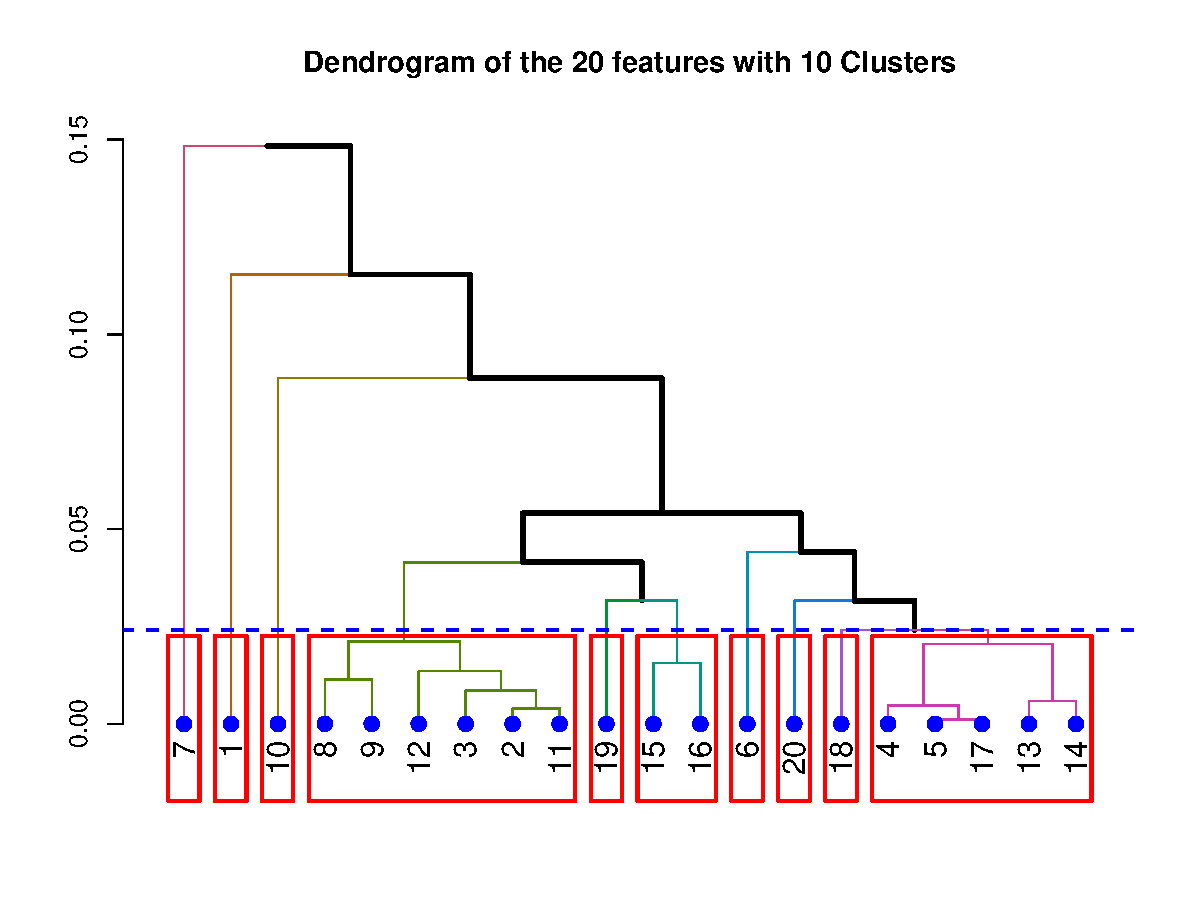
\includegraphics[scale=.75]{./images/cluster-10.pdf}
    \caption{Dendrogram with 10 clusters to select 1 features from each one}
    \label{fig:Cuthclust:10}
\end{figure}

Regarding the GPU parameters, we performed a correlation analysis and experimented with different number of parameters. As, it was not possible to get a high Spearman  Correlation Coefficient with the GPU parameters, the parameters were taken considering the order of the SCC. In this way, we compared the GPU parameters against the kernel execution times and tested with different number of GPU parameters. GPU parameters were 11 and during the experiments we concluded that few GPU parameters captured the relations between hardware and applications.


\begin{lstlisting}[basicstyle=\small,numbers=none]
[1]  compute_capability
[2]  gpu_clock_rate
[3]  num_of_cores
[4]  num_of_sm
[5]  num_sp_per_sm
[6]  L2_size
[7]  bus
[8]  memory_clock
[9]  theoretical_flops
[10] bandwidth
[11] global_memory_size
\end{lstlisting}

In these experiments, we used three different machine learning methods: Linear Regression, Support Vector Machines and Random Forest. These machine learning techniques achieved a high precision in the predictions with the extracted features. Ensemble methods were also tested, but the additional computational complexity did not justify the small improvement in accuracy of the predictions. We evaluate the ML algorithms using sets of 5 and 10 features, and considered two experimental contexts:

\begin{enumerate}
\item GPUs: we evaluated if the ML algorithm could predict the execution time over a previously unseen GPU. We used a leave-one-out cross validation procedure, by selecting the samples from one GPU as a test set and using the samples from the other 8 GPUs as training set.

\item Kernels: in this case we predict the execution time of a previously unseen CUDA kernel. We used the same leave-one-out cross validation procedure, but now selecting the samples from a single kernel as a test set and using the samples from the other 15 kernels as training set.
\end{enumerate}

